\documentclass[12pt]{article}
        \makeatletter
        \def\input@path{{../../}}
        \makeatother
        \usepackage{sbc-template}
        \makeatletter
        \renewcommand{\inst}[1]{}
        \makeatother
        \usepackage{graphicx,url}
        \usepackage[utf8]{inputenc}
        \usepackage[T1]{fontenc}
        \usepackage[brazil]{babel}
        \usepackage{longtable,booktabs,array}
        \usepackage{amsmath,amssymb}
        \providecommand{\tightlist}{%%
          \setlength{\itemsep}{0pt}\setlength{\parskip}{0pt}}
        \sloppy
        \title{Previsao de demanda e otimizacao de estoque: por que este problema importa}
        \author{}
        \address{}
        \begin{document}

        \maketitle

        \begin{resumo}
        Este primeiro artigo abre a série com o problema de negócio que vai sustentar todos os experimentos seguintes: previsão de demanda para reposição de estoque. O objetivo e mostrar por que esse problema e valioso, por que ele e difícil e por que ele cria um caminho didatico natural até Reservoir Computing (RC) e Quantum Reservoir Computing (QRC). Em vez de comecar pela teoria do reservatorio, comecamos pelo custo do erro no varejo, formalizamos a tarefa de previsão, fixamos o recorte experimental no dataset Favorita e mostramos as primeiras estatísticas reais da série \texttt{store\_nbr\ =\ 1} e \texttt{family\ =\ BEVERAGES}. Ao final, o leitor sabe como carregar o recorte, entende as métricas que vao guiar a série, enxerga o impacto de promocao e calendário e tem um mapa completo dos sete artigos.
        \end{resumo}

        \subsection{1. O que o leitor vai aprender}\label{1-o-que-o-leitor-vai-aprender}

Ao final deste artigo, você será capaz de:

\begin{enumerate}
\def\labelenumi{\arabic{enumi}.}
\tightlist
\item
  explicar por que previsão de demanda e um problema central de negócio;
\item
  formular matematicamente a tarefa de previsão da série;
\item
  reproduzir o recorte adotado no Favorita em toda a obra;
\item
  interpretar os primeiros artefatos computacionais antes de treinar qualquer modelo;
\item
  entender por que esse problema e uma boa rota pedagogica até QRC.
\end{enumerate}

\subsection{2. O problema de negócio antes do modelo}\label{2-o-problema-de-neguxf3cio-antes-do-modelo}

Previsao de demanda e importante porque o erro entra diretamente na decisao de estoque. Se a empresa compra menos do que deveria, perde venda. Se compra mais, imobiliza capital e aumenta o risco de desperdicio. Em um ambiente de varejo alimentar, isso acontece em escala diaria, com milhares de decisoes pequenas produzindo efeitos acumulados grandes.

Um modo simples de formalizar esse efeito e escrever o erro de previsão como

\[
e_{t+h} = y_{t+h} - \hat{y}_{t+h},
\]

em que \(y_{t+h}\) e a demanda observada e \(\hat{y}_{t+h}\) e a previsão produzida no tempo \(t\) para o horizonte \(h\).

Esse erro alimenta uma politica operacional mínima de reposição:

\[
R_t = \hat{y}_{t+1} + SS_t,
\]

em que \(R_t\) e a quantidade planejada para reposição e \(SS_t\) e um estoque de seguranca. Mesmo sem modelar toda a politica de inventario, a equação deixa claro o ponto principal: melhorar \(\hat{y}_{t+1}\) melhora a qualidade da decisao.

\subsection{3. Da pergunta de negócio para a tarefa de previsão}\label{3-da-pergunta-de-neguxf3cio-para-a-tarefa-de-previsuxe3o}

Ao longo da série, vamos modelar a tarefa como

\[
\hat{y}_{t+h} = f(y_{1:t}, x_{1:t+h}),
\]

em que:

\begin{itemize}
\tightlist
\item
  \(y_{1:t}\) representa o historico de vendas observado até o tempo \(t\);
\item
  \(x_{1:t+h}\) representa sinais exógenos, como promocao e calendário;
\item
  \(f(\cdot)\) será implementada por modelos estatísticos, de IA clássica, RC e QRC.
\end{itemize}

Essa forma e importante pedagogicamente porque nos permite manter o mesmo problema enquanto trocamos a família de modelo. O que muda do artigo 1 ao 7 não e a pergunta. O que muda e a maneira de construir a representação temporal.

\subsection{4. O dataset Favorita e o recorte didatico da série}\label{4-o-dataset-favorita-e-o-recorte-didatico-da-suxe9rie}

O projeto usa o dataset da competição \emph{Corporacion Favorita Grocery Sales Forecasting} como fio condutor. Para manter o ensino progressivo e reproduzivel, toda a série comeca no mesmo recorte:

\begin{itemize}
\tightlist
\item
  loja: \texttt{store\_nbr\ =\ 1}
\item
  família: \texttt{BEVERAGES}
\item
  frequencia: diaria
\item
  teste: ultimos \texttt{90} dias
\end{itemize}

A tabela abaixo resume o recorte real usado nas implementações.

\begin{longtable}[]{@{}ll@{}}
\toprule\noalign{}
Metrica & Valor \\
\midrule\noalign{}
\endhead
\bottomrule\noalign{}
\endlastfoot
Dias totais no recorte & 1688 \\
Dias de treino & 1598 \\
Dias de teste & 90 \\
Media diaria de vendas & 1583.99 \\
Desvio padrao das vendas & 729.89 \\
Taxa média de promocao & 60.37\% \\
Taxa de dias com venda zero & 0.59\% \\
Inicio do treino & 2013-01-01 \\
Inicio do teste & 2017-05-18 \\
Fim do teste & 2017-08-15 \\
\end{longtable}

O carregamento desse recorte e implementado em \texttt{code/common/favorita.py}. O nucleo da reproducao e o seguinte:

\begin{verbatim}
from common.favorita import (
    FavoritaSeriesConfig,
    load_store_family_series,
    temporal_train_test_split,
)

config = FavoritaSeriesConfig(store_nbr=1, family="BEVERAGES", test_days=90)
frame = load_store_family_series(store_nbr=config.store_nbr, family=config.family)
train, test = temporal_train_test_split(frame, test_days=config.test_days)
\end{verbatim}

Esse codigo faz três coisas que sao centrais para toda a série:

\begin{enumerate}
\def\labelenumi{\arabic{enumi}.}
\tightlist
\item
  fixa um recorte comum para todos os modelos;
\item
  densifica o calendário diario, preenchendo dias faltantes com zero;
\item
  garante um split temporal identico para comparações posteriores.
\end{enumerate}

\subsection{5. O que os dados já ensinam antes de qualquer modelo}\label{5-o-que-os-dados-juxe1-ensinam-antes-de-qualquer-modelo}

Antes de falar de RC ou QRC, vale observar o comportamento bruto da série.

\pandocbounded{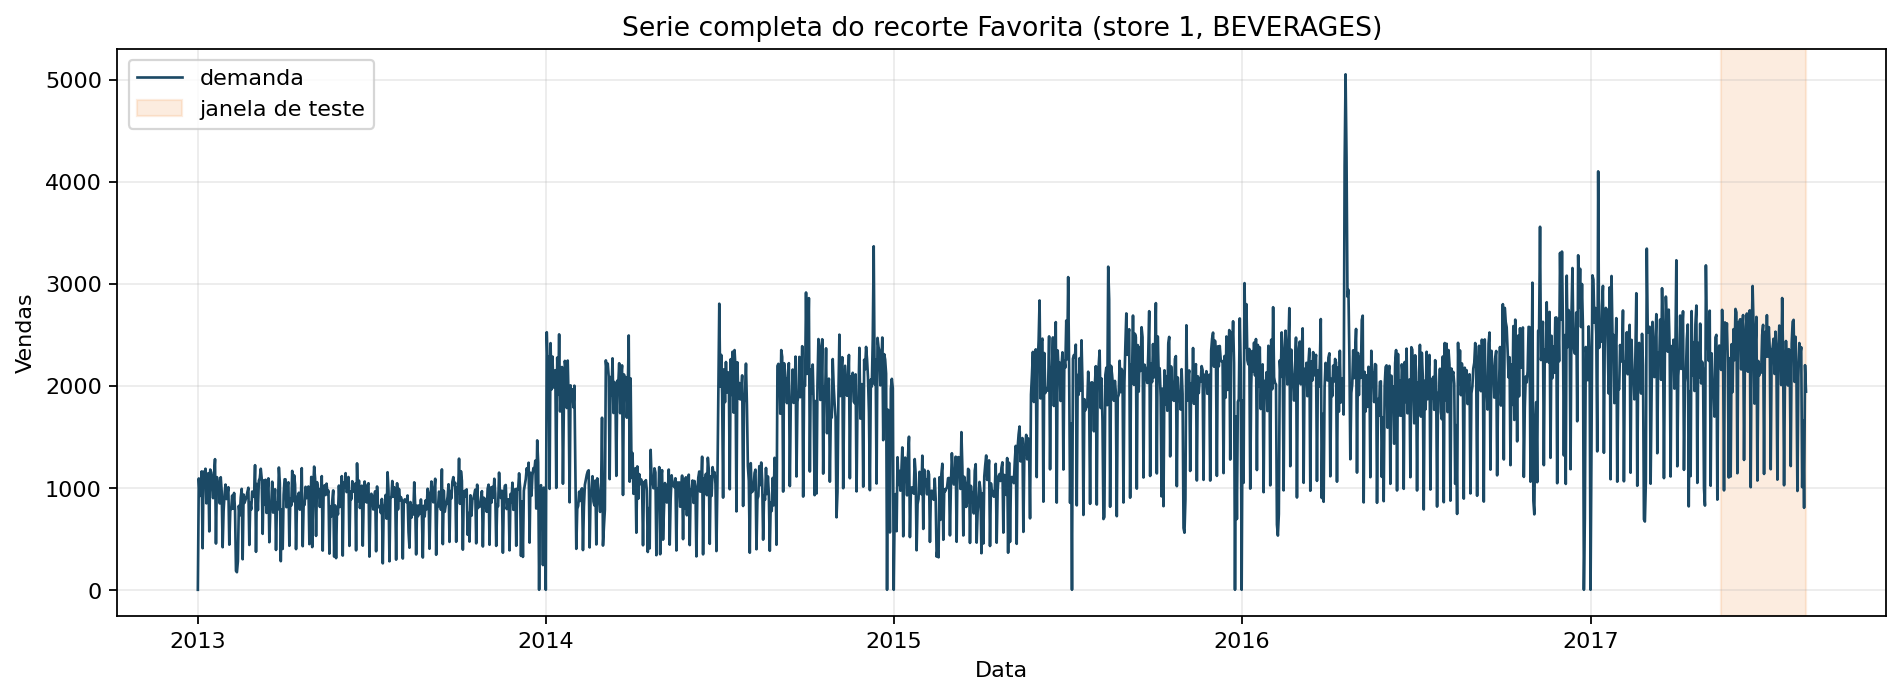
\includegraphics[keepaspectratio,alt={Visao geral da série de demanda usada ao longo da série de artigos.}]{computational_results_20260402_222902/series_overview.png}}

A visao geral mostra que o problema não e trivial por pelo menos três motivos:

\begin{itemize}
\tightlist
\item
  há variacao forte ao longo do tempo;
\item
  a série responde a padroes semanais;
\item
  promocao altera o patamar das vendas.
\end{itemize}

O perfil semanal medio confirma esse ultimo ponto.

\begin{longtable}[]{@{}lll@{}}
\toprule\noalign{}
Dia da semana & Media com promocao & Media sem promocao \\
\midrule\noalign{}
\endhead
\bottomrule\noalign{}
\endlastfoot
Monday & 2074.45 & 1125.28 \\
Tuesday & 2016.35 & 1046.04 \\
Wednesday & 2248.32 & 1166.31 \\
Thursday & 1927.36 & 1074.45 \\
Friday & 2116.13 & 1133.84 \\
Saturday & 2209.90 & 1232.53 \\
Sunday & 977.32 & 498.80 \\
\end{longtable}

\pandocbounded{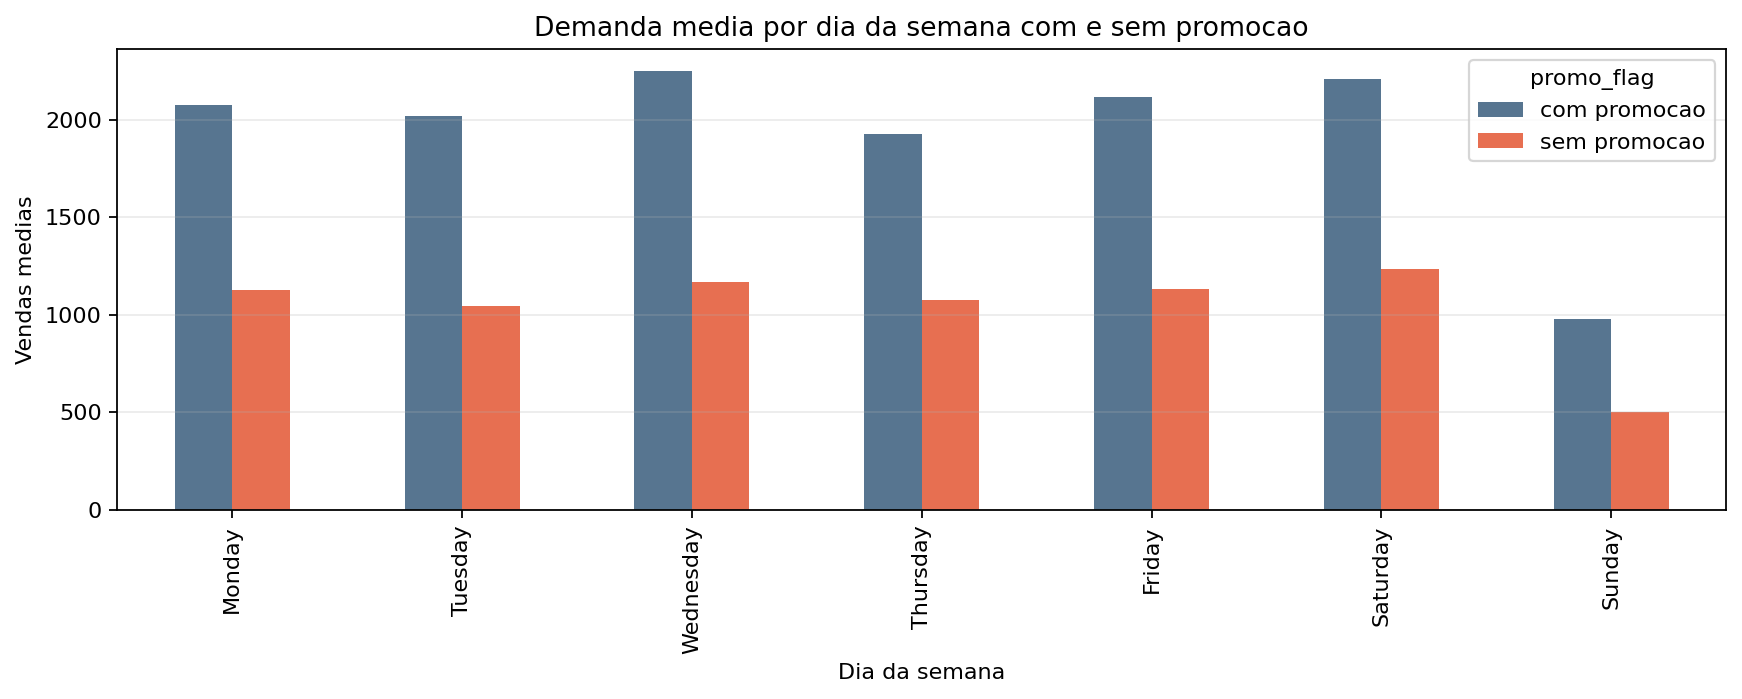
\includegraphics[keepaspectratio,alt={Perfil semanal medio com e sem promocao no recorte adotado.}]{computational_results_20260402_222902/weekly_profile.png}}

Duas leituras didaticas aparecem imediatamente:

\begin{enumerate}
\def\labelenumi{\arabic{enumi}.}
\tightlist
\item
  a série tem sazonalidade semanal clara, o que justifica baselines como \texttt{Seasonal\ Naive} e \texttt{ETS};
\item
  promocao desloca a média de vendas em todos os dias da semana, o que torna natural incluir variáveis exógenas.
\end{enumerate}

Esse e o primeiro motivo para escolher esse problema como rota até QRC: mesmo o recorte inicial já exige memoria temporal e sensibilidade a contexto.

\subsection{6. Passo-a-passo para reproduzir o recorte}\label{6-passo-a-passo-para-reproduzir-o-recorte}

O leitor pode reproduzir o ponto de partida da obra em quatro passos.

\subsubsection{6.1 Passo 1: localizar os dados}\label{61-passo-1-localizar-os-dados}

Os arquivos brutos foram organizados em \texttt{dataset/raw/}, com \texttt{train.csv}, \texttt{transactions.csv}, \texttt{stores.csv}, \texttt{holidays\_events.csv}, \texttt{oil.csv} e \texttt{test.csv}.

\subsubsection{6.2 Passo 2: carregar uma unica série}\label{62-passo-2-carregar-uma-unica-suxe9rie}

A função \texttt{load\_store\_family\_series()} filtra por loja e família, ordena por data e produz um \texttt{DataFrame} com as colunas:

\begin{itemize}
\tightlist
\item
  \texttt{ds}: data
\item
  \texttt{y}: demanda diaria
\item
  \texttt{onpromotion}: sinal exógeno básico usado nos modelos
\end{itemize}

\subsubsection{6.3 Passo 3: fixar o split temporal}\label{63-passo-3-fixar-o-split-temporal}

A função \texttt{temporal\_train\_test\_split()} implementa a regra que vamos herdar em toda a série:

\begin{itemize}
\tightlist
\item
  o passado vai para treino;
\item
  os ultimos \texttt{90} dias vao para teste;
\item
  nenhuma observacao do futuro entra no treino.
\end{itemize}

\subsubsection{6.4 Passo 4: inspecionar o recorte}\label{64-passo-4-inspecionar-o-recorte}

Os artefatos computacionais deste artigo já mostram o mínimo necessario para não modelar no escuro:

\begin{itemize}
\tightlist
\item
  \texttt{series\_overview.png}
\item
  \texttt{weekly\_profile.png}
\item
  \texttt{recorte\_summary.csv}
\end{itemize}

Em um projeto real, essa etapa não e opcional. Ela evita treinar modelos sofisticados sobre uma série mal definida.

\subsection{7. Como vamos medir desempenho}\label{7-como-vamos-medir-desempenho}

Toda a obra usa as mesmas quatro métricas, implementadas em \texttt{code/common/metrics.py}.

O erro absoluto medio e dado por

\[
\mathrm{MAE} = \frac{1}{n} \sum_{t=1}^n |y_t - \hat{y}_t|.
\]

O erro quadrático medio com raiz e dado por

\[
\mathrm{RMSE} = \sqrt{\frac{1}{n} \sum_{t=1}^n (y_t - \hat{y}_t)^2}.
\]

O erro absoluto ponderado pelo volume da série e dado por

\[
\mathrm{WAPE} = \frac{\sum_{t=1}^n |y_t - \hat{y}_t|}{\sum_{t=1}^n |y_t|}.
\]

E o erro percentual absoluto medio simetrico e dado por

\[
\mathrm{sMAPE} = \frac{1}{n} \sum_{t=1}^n
\frac{2 |y_t - \hat{y}_t|}{|y_t| + |\hat{y}_t|}.
\]

Essas métricas vao aparecer repetidamente porque cada uma responde a uma pergunta diferente:

\begin{itemize}
\tightlist
\item
  \texttt{MAE}: erro medio em unidades de venda;
\item
  \texttt{RMSE}: sensibilidade a erros grandes;
\item
  \texttt{WAPE}: erro relativo ao volume total;
\item
  \texttt{sMAPE}: comparação percentual mais estável em séries com escalas diferentes.
\end{itemize}

\subsection{8. Por que esse problema conduz naturalmente até RC e QRC}\label{8-por-que-esse-problema-conduz-naturalmente-atuxe9-rc-e-qrc}

Ha pelo menos quatro motivos.

\begin{enumerate}
\def\labelenumi{\arabic{enumi}.}
\tightlist
\item
  A série depende do passado, entao memoria importa.
\item
  O efeito de promocao e calendário não e constante, entao não linearidade importa.
\item
  O protocolo de negócio e simples de explicar, entao o leitor não se perde no dominio.
\item
  O mesmo recorte pode ser usado para modelos estatísticos, IA clássica, RC e QRC.
\end{enumerate}

Em outras palavras, o problema e suficientemente real para ser relevante e suficientemente controlado para ser didatico.

\subsection{9. Roadmap dos sete artigos}\label{9-roadmap-dos-sete-artigos}

O percurso da série será o seguinte:

\begin{enumerate}
\def\labelenumi{\arabic{enumi}.}
\tightlist
\item
  artigo 1: problema de negócio, recorte e métricas;
\item
  artigo 2: fundamentos de Reservoir Computing;
\item
  artigo 3: primeiro pipeline reproduzivel com baseline e RC;
\item
  artigo 4: memoria, não linearidade e tuning do RC;
\item
  artigo 5: benchmark justo entre todas as implementações;
\item
  artigo 6: ponte de RC clássico para QRC;
\item
  artigo 7: estudo final de QRC no Favorita.
\end{enumerate}

Essa organização evita um erro comum em textos de QRC: apresentar o formalismo quântico antes de o leitor entender a tarefa, o protocolo experimental e a lógica do reservatorio.

\subsection{10. Conclusao}\label{10-conclusao}

O ponto de partida da série esta estabelecido. Temos um problema de negócio real, um recorte experimental fixo, um pipeline mínimo de carregamento de dados e um conjunto de métricas que permitira comparações honestas. Esse chao comum e o que torna possível ensinar RC e QRC sem perder o leitor em abstrações.

O próximo artigo parte daqui para responder a pergunta central que o leitor provavelmente já esta fazendo: afinal, o que e um reservatorio e por que ele pode ser útil para uma série temporal como essa?

\subsection{Entregaveis associados no repositorio}\label{entregaveis-associados-no-repositorio}

\begin{itemize}
\tightlist
\item
  dados brutos: \texttt{dataset/raw/}
\item
  carga do recorte: \texttt{code/common/favorita.py}
\item
  métricas: \texttt{code/common/metrics.py}
\item
  artefatos deste artigo: \texttt{computational\_results\_20260402\_222902/}
\item
  figuras principais: \texttt{series\_overview.png} e \texttt{weekly\_profile.png}
\end{itemize}

\subsection{Referencias}\label{referencias}

\begin{itemize}
\tightlist
\item
  Corporacion Favorita Grocery Sales Forecasting. Kaggle.
\item
  Hyndman, R. J.; Athanasopoulos, G. Forecasting: Principles and Practice.
\item
  Jaeger, H. The "echo state" approach to analysing and training recurrent neural networks.
\item
  Lukosevicius, M.; Jaeger, H. Reservoir computing approaches to recurrent neural network training.
\end{itemize}

        \end{document}
